\subtitle{Emiiones en rellenos sanitarios}
\begin{frame}
  \titlepage
\end{frame}
% Uncomment these lines for an automatically generated outline.
%\begin{frame}{Outline}
%  \tableofcontents
%\end{frame}

\section{Introducción}

\begin{frame}{Descripción del transporte}


Dos formas \textit{equivalentes} de pensar el problema: 
\begin{itemize}
    \item Descripción \alert{Lagrangiana} ó enfoque \textit{material}: Estudiar como se mueve un contaminante en el tiempo y espacio.
    
    \item Descripción \alert{Euleriana} ó enfoque de \textit{campos}: Estudiar como cambia con el tiempo la concentración de un contaminante en el espacio.
    
\end{itemize}

\begin{center}
    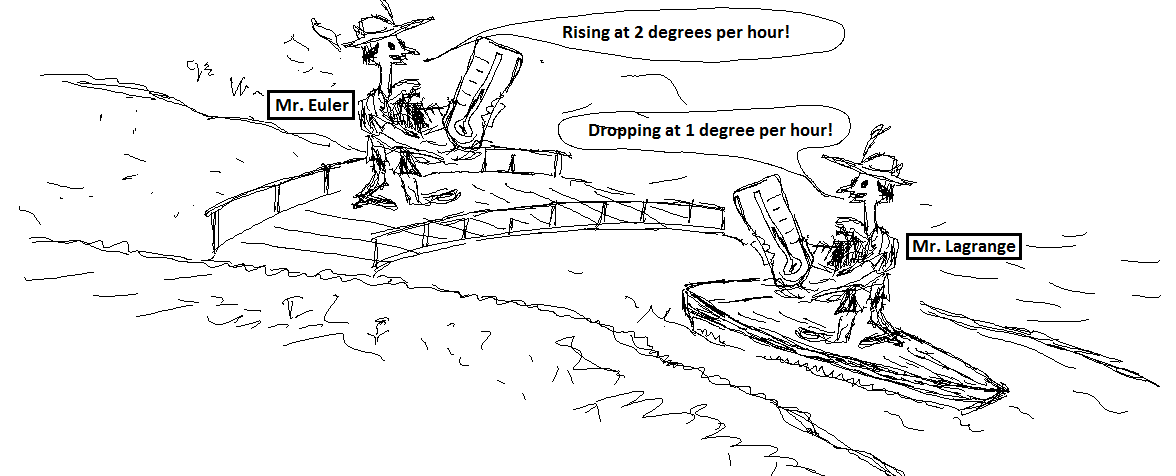
\includegraphics[width=0.6\textwidth]{img/MaterialDerivative.png}
\end{center}

En este curso vamos a adoptar la descripción \textbf{Euleriana}.
    
\end{frame}
